\chapter{Transfer learning}
\label{chap:transfer-learning}

Les approches du transfer Learning (TL) sont nombreuses. Cependant, les premières techniques de TL faisaient hypothèse qu'il existe un lien entre les images de la source et celles de la destination. Cela pouvait être une similarité de classe, par exemple de la salade en sources et des soupes en destination qui sont tout deux de la nourriture, ou des caractéristiques communes. Par exemple, des vélos en sources et des trottinettes en destination qui ont tout deux des roues.

L'idée étant que certaines couches contiennent en elles l'extraction et l'identification de ces caractéristique, le but est d'exploiter au mieux ces couches afin de pouvoir entraîner plus rapidement ou plus efficacement un modèle pour une nouvelle tâche.

Chaque spécialisation de transfer learning va donc correspondre à un enjeux bien particulier.

\section{Multi-data Transfer Learning}
\label{sec:multi-data}
Afin de pallier le problème du manque de données, une approche est de multiplier les bases de données afin de profiter de l'apprentissage de certaines caractéristiques dans le réseau, soit en profitant de plusieurs sources, soit en exploitant les similarités d'un même apprentissage sur différents domaines.

\subsection{Multi-sources TL}
\label{subsec:multi-sources}

Le Multi-source Transfer Learning \cite{multi-source} est une méthode qui consiste à essayer d'effacer les différences de caractéristiques entre le domaine source et une destination en multipliant les sources. On va donc disposer, avec ce genre de méthodes, de $N$ sources avec lesquelles on va entraîner $N$ réseaux. Chaque réseau va disposer de couches extractrices de caractéristiques et de couches classifieurs. Dans le réseau final, les $N$ couches d'extractions sont rassemblées ensemble et on fait de même avec les couches de classifications.

Ensuite, une fois que l'on a obtenu ce réseau final, il va être entraîné avec les données de destination de manière classique.

\subsection{Multi-tasking Learning}
\label{subsec:multi-tasking}

Le multi-tasking Learning est une méthode qui consiste à appliquer plusieurs traitements à une même image. Par exemple, segmenter l'image en fonction des profondeurs ou générer l'image des normales. Du fait que l'on parte d'une même source pour ces images, on va pouvoir calculer la similarité entre une tâche et les autres. Les réseaux des différentes tâches vont être séparés mais vont prendre en compte des éléments des autres réseaux dans leur fonction de coût et leur fonction d'optimisation.

L'apprentissage est ainsi réparti entre chaque réseau tout en faisant en sorte que chaque réseau soit spécialisé dans une seule tâche.

La méthode de multi-tasking la plus complète est celle de Stanford appelé "Taskonomie" \cite{tasknomie-presentation}. Le score de similarité entre tâches est calculé à partir d'une méthode inspirée des neurosciences appelées RSA (Representation Similarity Analysis). Il est créé une matrice des similarités qui donne une vue globale des correspondances entre chaque tâche et les autres. La matrice est le résultat de l'application directe du calcul RSA entre chaque couple de base de données. Les fonctions de coût des réseaux des $N$ tâches vont prendre en compte la matrice de similarité. Ainsi, chaque tâche va prendre en compte la progression d'une tâche qui est proche d'elle.

Cela nécessite plus de contraintes sur les données que le multi-source car toutes les destinations doivent être liées à la même source. La base de données la plus complète que nous avons trouvée est celle de Stanford qui propose 15 destinations pour une même source \cite{zamir2018taskonomy}.

Cependant cette méthode ne réduit pas le nombre de données par tâche. Par contre, l'entraînement commun permet une convergence plus rapide et un taux de réussite plus grand que si les tâches sont entraînées individuellement.


\section{Deep Learning Transfer}
\label{sec:deepT}

Les travaux catégorisés en tant que "Deep Learning en TL" sont les travaux qui vont se focaliser sur un réseau en particulier (resnet, YOLO, etc) ou un réseau et une tâche particulière et expliquer quelles sont les couches à enlever/modifier ou les fonctions de coût optimum à utiliser avec ce réseau.

Les réseaux Deep étant actuellement beaucoup utilisés, de nombreux articles \cite{Sun2019ExploringBF, DBLP:journals/corr/abs-1804-06275, 8729686, 7966162} sont basés sur ces approches et cherchent à optimiser leurs résultats par rapport à ceux de travaux déjà existants sur des problèmes similaires. Comme dit précédemment, l'optimisation peut porter sur les couches à remplacer ou ajouter, la fonction de coût ou d'optimisation mais aussi sur la base de données source à utiliser.

Comme on peut le voir sur la figure \ref{fig:features-extract}, les couches basses (proches de l'entrée), vont contenir des données de bas niveau, généralement du filtrage ou de l'extraction de contours. Les couches suivantes vont avoir tendance à se spécialiser dans l'extraction de donner liées aux images fournies. Par exemple, pour la reconnaissance de visages, on voit sur la figure \ref{fig:features-extract} que les couches moyennes reconnaissent des parties de visages (nez, bouche, yeux) et les couches de haut niveau des visages en entier. Le but est donc, pour une tâche particulière, d'identifier les couches "génériques" dont on va vouloir se resservir pour un nouvel apprentissage et quelle est la partie du modèle que l'on ne peut pas garder.

\begin{figure}[!h]
\centering
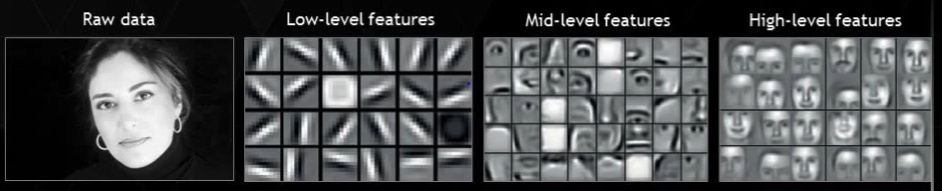
\includegraphics[scale=0.5]{img/features.png}
\caption{Visualisation des descripteurs des couches de bas, moyen et haut niveaux \cite{featureGFaces}}
\label{fig:features-extract}
\end{figure}

Ainsi l'article \cite{Kornblith_2019_CVPR} compare l'efficacité de l'utilisation des bases de données les plus utilisées en tant que source. Les sources les plus utilisées sont ImageNet, COCO, CIFAR et FOOD-101 car elles contiennent plusieurs dizaines de milliers, voire des millions d'images, ce qui les rend intéressantes en tant que sources. Ces sources peuvent, cependant, être éloignées des données de destination. Il est donc nécessaire de faire des tests et de comparer afin de savoir quelles bases de données seront les meilleures pour les cas choisis.

\subsection*{Le cas particulier des réseaux adverses}
\label{subsec:adversials}
Les réseaux deep avec adversial sont un type de réseau particulier. En plus de l'apprentissage d'un réseau profond classique, un deuxième réseau, \textit{l'adversaire} (ou \textit{l'adversial}), est mis à coté du premier et à pour rôle de critiquer l'apprentissage du premier. Le but de cette critique peut être de rendre une classification résistante à des attaques ou de maximiser un critère d'apprentissage précis.

Dans cette optique, des méthodes ont été proposées afin de se servir des réseaux adverses dans le cas du transfer learning et le \textit{Deep Learning Transfer avec Adversial} est une sous-catégorie à part entière du simple \textit{Deep Learning Transfer}.

Le papier le plus intéressant dans cette optique a été celui qui présente les Joint Adaptation Networks (JAN) \cite{DBLP:journals/corr/Long0J16a}, dont l'intérêt et de proposer une version du réseau sans adversaire et une version avec adversaire, appeler JAN-A. Le réseau adverse sert à calculer un critère de minimisation le joint maximum Mean Discrepancy (JMMD). Ce critère représente la distribution conjointe entre la source et la destination. En somme, le but de l'adversaire va être de calculer la distribution conjointe (les points communs) entre les données apprises de la base source et les données de la destination.

Cela permet de récupérer de manière plus efficace sur les caractéristiques communes entre la source et la destination. Le calcul de quelles features garder sera fait directement par le réseau.
Le taux d'apprentissage sur des données ne contenant que 600 images sera équivalent à celui entraîner sur des données en contenant plusieurs milliers.
